Seluruh program ditulis dalam Python dan berada di folder \texttt{src/}. Bab ini
menjelaskan representasi persoalan, heuristik yang dipakai bersama oleh semua
algoritma, lalu implementasi setiap algoritma. Potongan kode diambil langsung dari
\textit{repository}.

\section{Struktur Program}

\begin{table}[H]
	\centering
	\caption{Modul program}
	\label{tab:modul}
	\begin{tabular}{l p{8.3cm}}
		\toprule
		\textbf{Modul} & \textbf{Isi} \\
		\midrule
		\texttt{core/models.py} & Data statis: \texttt{Package}, \texttt{Truck}, \texttt{Problem} \\
		\texttt{core/validation.py} & Validasi tipe dan rentang parameter serta data instans \\
		\texttt{core/state.py} & Representasi \textit{state}: \texttt{Placement} dan \texttt{State} \\
		\texttt{core/orientation.py} & Enam orientasi paket dan rotasi $90^\circ$ \\
		\texttt{core/geometry.py} & Operasi balok: tumpang tindih, tumpuan, dinding \\
		\texttt{core/constraints.py} & Pendeteksian pelanggaran batasan \\
		\texttt{core/objective.py} & Fungsi objektif \textit{value} dan ETA \\
		\texttt{core/repair.py} & Heuristik \textit{repair} \textit{state} menjadi valid \\
		\texttt{core/neighbors.py} & Aksi \textit{swap}, \textit{move}, \textit{rotate} dan pembangkit tetangga \\
		\texttt{core/initial.py} & \textit{State} awal acak \\
		\texttt{core/bounds.py} & Batas atas optimum global (\textit{knapsack}) \\
		\texttt{core/io.py}, \texttt{core/result.py} & Baca/tulis instans dan hasil \textit{run} (JSON) \\
		\texttt{algorithms/} & Hill-Climbing, Simulated Annealing, Genetic Algorithm \\
		\texttt{experiments/} & Skrip eksperimen HC, SA, dan GA \\
		\texttt{viz/} & Visualisasi 3D \textit{state} dan plot hasil eksperimen \\
		\texttt{main.py} & Antarmuka baris perintah untuk satu kali \textit{run} \\
		\bottomrule
	\end{tabular}
\end{table}

\section{Representasi State}

Data paket dan truk tidak berubah selama pencarian, sehingga dipisahkan dari
\textit{state}. Sebuah \textit{state} adalah \textit{tuple} berisi satu
\texttt{Placement} untuk setiap paket, berurutan sesuai indeks paket. \texttt{Placement}
menyimpan apakah paket berada di dalam truk, koordinat sudut kiri-bawah-belakang
$(x,y,z)$, dan orientasinya. Orientasi ditulis seperti pada spesifikasi, yaitu sumbu
truk yang sejajar dengan sisi \texttt{w}, \texttt{l}, dan \texttt{h}; misalnya
\texttt{("y","x","z")} berarti \{w:y, l:x, h:z\}. Karena semua objek bersifat
\textit{immutable} (\texttt{frozen=True}), \textit{state} dapat langsung dibandingkan
dan disimpan di dalam \textit{set}.

\lstinputlisting[caption={Model persoalan (\texttt{src/core/models.py})},linerange={11-60}]{../src/core/models.py}
\lstinputlisting[caption={Representasi \textit{state} (\texttt{src/core/state.py})}]{../src/core/state.py}

\section{Batasan dan Fungsi Objektif}

\texttt{find\_violations} memeriksa kelima batasan untuk semua paket di dalam truk.
Balok direpresentasikan sebagai interval setengah terbuka $[x_0,x_1)$, sehingga dua
paket yang hanya bersentuhan sisi tidak dianggap bertumpuk. Fungsi
\texttt{rests\_on} mengikuti definisi tumpuan pada spesifikasi: paket atas tepat
berada di permukaan atas paket bawah dan proyeksi alasnya beririsan.

\lstinputlisting[caption={Pemeriksaan batasan (\texttt{src/core/constraints.py})},linerange={16-67}]{../src/core/constraints.py}

Fungsi objektif adalah total \textit{value} paket di dalam truk. Modul ini juga
menyediakan \texttt{evaluate}, yaitu \textit{value} dikurangi penalti sebesar
(\textit{value} paket termahal $+\,1$) untuk setiap pelanggaran. Dengan penalti tersebut,
memasukkan paket secara ilegal tidak pernah lebih menguntungkan daripada
mengeluarkannya. Namun ketiga algoritma pada akhirnya selalu bekerja pada
\textit{state} yang sudah di-\textit{repair} (Subbab~\ref{sec:repair}), sehingga nilai
objektif yang dilaporkan sama dengan total \textit{value} \textit{state} valid.

\lstinputlisting[caption={Fungsi objektif (\texttt{src/core/objective.py})},linerange={24-44}]{../src/core/objective.py}

\section{Heuristik Repair}
\label{sec:repair}

\textit{State} awal acak dan sebagian besar tetangga acak melanggar batasan
(paket melayang atau bertumpuk). Agar pencarian selalu berada di ruang solusi valid,
setiap \textit{state} dilewatkan ke \texttt{repair}. Heuristik ini deterministik dan
hanya \emph{mengeluarkan} atau \emph{menurunkan} paket, tidak pernah menambah paket,
sehingga peningkatan nilai tetap berasal dari algoritma pencarian. Langkahnya:
\begin{enumerate}
	\item Paket yang menembus dinding dikeluarkan dari truk.
	\item Selama total berat melebihi kapasitas, paket dengan rasio
	\textit{value}/berat terendah dikeluarkan.
	\item Paket diproses dari bawah ke atas (urut $z$, lalu \textit{value} terbesar).
	Paket yang bertumpuk dengan paket yang sudah diterima dikeluarkan. Paket lain
	``dijatuhkan'' ke permukaan tertinggi di bawahnya (atau lantai), seperti gravitasi.
	Jika permukaan tempatnya mendarat adalah paket \textit{fragile}, paket dikeluarkan.
\end{enumerate}

\lstinputlisting[caption={Heuristik \textit{repair} untuk satu truk (\texttt{src/core/repair.py})},linerange={38-78}]{../src/core/repair.py}

\section{Aksi Tetangga}

Ketiga aksi pada spesifikasi diimplementasikan sebagai fungsi murni yang
mengembalikan \textit{state} baru:
\texttt{move} memindahkan paket ke koordinat lain atau ke luar truk,
\texttt{rotate} memutar paket $90^\circ$ terhadap suatu sumbu (dua sumbu lainnya
bertukar), dan \texttt{swap} menukar posisi dua paket (masing-masing tetap dengan
orientasinya).

\lstinputlisting[caption={Aksi \textit{move}, \textit{rotate}, dan \textit{swap} (\texttt{src/core/neighbors.py})},linerange={28-54}]{../src/core/neighbors.py}

Ruang koordinat bilangan bulat sangat besar, sedangkan kebanyakan koordinat acak
menghasilkan paket melayang. Karena itu, tujuan aksi \textit{move} diambil dari
\textit{extreme points}~\cite{crainic2008extreme}: titik asal dan titik di kanan,
depan, serta atas setiap paket yang sudah ada di truk, selama paket masih muat di
dalam dinding. Tetangga acak (\texttt{random\_neighbor}) memilih jenis aksi secara
seragam. Untuk \textit{move}, paket di dalam truk dikeluarkan dengan peluang 0,2;
selain itu tujuannya diambil dari \textit{extreme point} (peluang 0,5) atau dari
koordinat acak di dalam dinding. \texttt{all\_neighbors} membangkitkan semua tetangga
untuk \textit{steepest-ascent}: semua rotasi, semua \textit{swap} yang mengubah
sesuatu, serta semua \textit{move} ke luar truk dan ke setiap \textit{extreme point}.

\lstinputlisting[caption={\textit{Extreme points} dan tetangga acak (\texttt{src/core/neighbors.py})},linerange={56-121}]{../src/core/neighbors.py}

\section{State Awal}

Sesuai spesifikasi, \textit{state} awal dibangkitkan acak: setiap paket mendapat
orientasi acak dan, dengan peluang 0,5, dimasukkan ke truk pada koordinat acak di
dalam dinding. \textit{State} ini umumnya tidak valid, lalu di-\textit{repair} oleh
setiap algoritma.

\lstinputlisting[caption={\textit{State} awal acak (\texttt{src/core/initial.py})},linerange={13-32}]{../src/core/initial.py}

\section{Batas Atas Optimum Global}
\label{sec:bound}

Optimum global sebenarnya tidak diketahui. Untuk menilai seberapa dekat hasil setiap
algoritma, dihitung batas atas berupa \textit{knapsack} 0/1 dengan dua batasan, yaitu
berat (kapasitas truk) dan volume (volume peti kemas), yang diselesaikan secara tepat
dengan \textit{dynamic programming}~\cite{martello1990knapsack}. Relaksasi ini
mengabaikan geometri, sehingga nilainya selalu $\ge$ optimum global. Besaran
$\text{gap} = 1 - f(s)/\text{batas atas}$ merupakan batas atas jarak hasil ke optimum
global.

\lstinputlisting[caption={Batas atas \textit{knapsack} (\texttt{src/core/bounds.py})},linerange={14-32}]{../src/core/bounds.py}

\section{Hill-Climbing}

Semua varian Hill-Climbing diimplementasikan di \path{src/algorithms/hill_climbing.py}
(bonus). Setiap tetangga di-\textit{repair} sebelum dinilai. Parameter yang dipakai
pada eksperimen: \texttt{max\_iterations}=100, \texttt{neighbor\_samples}=50 untuk
\textit{stochastic}, \texttt{max\_sideways}=20, dan \texttt{max\_restarts}=5 (instans
\textit{large} memakai 2 karena waktu eksekusinya lama).

\begin{itemize}
	\item \textbf{Steepest-ascent} memakai \texttt{\_best\_neighbor}, yang menilai seluruh
	\texttt{all\_neighbors}. Berhenti jika tetangga terbaik tidak lebih baik.
	\item \textbf{Stochastic} memilih secara acak salah satu tetangga yang lebih baik.
	Untuk menghemat waktu, mula-mula diambil 50 tetangga acak. Jika tidak ada yang lebih
	baik, seluruh \texttt{all\_neighbors} diperiksa dan salah satu tetangga yang lebih baik
	dipilih secara seragam. Pencarian berhenti hanya jika tidak ada satu pun tetangga yang
	lebih baik (\textit{local optimum}) atau \texttt{max\_iterations} tercapai.
	\item \textbf{Sideways move} seperti \textit{steepest-ascent}, tetapi boleh pindah ke
	tetangga bernilai sama yang belum pernah dikunjungi. Berhenti ketika banyak
	\textit{sideways move} mencapai \texttt{max\_sideways}. Karena tetangga bernilai sama
	yang sudah dikunjungi tidak dipilih lagi, pencarian tidak dapat berputar dalam siklus.
	\item \textbf{Random-restart} menjalankan \textit{steepest-ascent} dari \textit{state}
	awal acak sebanyak \texttt{max\_restarts}$+1$ kali dan mengambil hasil terbaik.
	Banyak iterasi per \textit{restart} dicatat.
\end{itemize}

\lstinputlisting[caption={Satu kali pendakian Hill-Climbing (\texttt{src/algorithms/hill\_climbing.py})},linerange={109-171}]{../src/algorithms/hill_climbing.py}

\section{Simulated Annealing}

Simulated Annealing diimplementasikan di \path{src/algorithms/simulated_annealing.py}.
Setiap iterasi mengambil satu tetangga acak yang sudah di-\textit{repair}. Tetangga
diterima jika $\Delta E\ge 0$; jika tidak, diterima dengan peluang $e^{\Delta E/T}$.
Heuristik yang dipakai:
\begin{itemize}
	\item \textbf{Kalibrasi suhu awal.} Jika $T_0$ tidak diberikan, diambil 100 tetangga
	acak dari \textit{state} awal dan dihitung rata-rata $|\Delta E|$ langkah yang
	memburuk, lalu $T_0=-\overline{|\Delta E|}/\ln p_0$. Dengan begitu, langkah memburuk
	rata-rata diterima dengan peluang $p_0$ di awal pencarian~\cite{benameur2004t0}.
	\item \textbf{Jadwal dengan titik ujung tetap.} Iterasi pertama memakai $T_0$ dan iterasi
	terakhir tepat $T_{\min}$, secara geometrik ($T_k=T_0(T_{\min}/T_0)^{k/(n-1)}$,
	$k=0,\dots,n-1$) atau linear.
	Banyak iterasi menjadi satu-satunya parameter biaya.
	\item \textbf{Simpan \textit{state} terbaik.} Hasil akhir adalah \textit{state} terbaik
	yang pernah dikunjungi, bukan \textit{state} terakhir.
	\item \textbf{Ratio swap (opsional).} Dengan peluang \texttt{ratio\_bias}, tetangga yang
	diusulkan adalah \textit{swap} antara paket di dalam truk yang rasio
	\textit{value}/beratnya rendah dan paket di luar yang rasionya tinggi. Aksinya
	tetap \textit{swap} biasa; hanya pemilihan paketnya yang dibias.
	\item \textbf{Definisi \textit{stuck}.} SA dianggap \textit{stuck} di \textit{local optimum}
	jika nilai objektif \textit{state} sekarang tidak berubah selama 500 iterasi
	berturut-turut. Satu \textit{plateau} dihitung satu kali.
\end{itemize}

\lstinputlisting[caption={Kalibrasi $T_0$, jadwal suhu, dan peluang penerimaan (\texttt{src/algorithms/simulated\_annealing.py})},linerange={48-66,94-106}]{../src/algorithms/simulated_annealing.py}
\lstinputlisting[caption={Iterasi utama Simulated Annealing (\texttt{src/algorithms/simulated\_annealing.py})},linerange={110-189}]{../src/algorithms/simulated_annealing.py}

\section{Genetic Algorithm}
\label{sec:ga-impl}

Genetic Algorithm diimplementasikan di \path{src/algorithms/genetic.py} mengikuti
salindia kuliah~\cite{kkif2026slides}:
\begin{itemize}
	\item \textbf{Individu} adalah satu \textit{state} lengkap; gen ke-$i$ adalah
	\texttt{Placement} paket ke-$i$.
	\item \textbf{Populasi awal} berisi $k$ \textit{state} acak yang di-\textit{repair}.
	\item \textbf{Fitness} adalah total \textit{value} (fungsi objektif).
	\item \textbf{Seleksi} memakai \textit{roulette wheel} (\texttt{roulette\_select}).
	\item \textbf{Crossover} memakai \textit{single-point crossover}: titik potong acak di
	$[1,n-1]$, kedua induk bertukar ekor sehingga terbentuk dua anak.
	\item \textbf{Mutasi}: dengan peluang 0,2, anak dikenai satu aksi tetangga acak
	(\textit{move}/\textit{rotate}/\textit{swap}).
\end{itemize}
Ada tiga adaptasi terhadap versi salindia. Pertama, setiap anak di-\textit{repair},
karena hasil \textit{crossover} dapat bertumpuk atau melayang. Kedua, satu individu
terbaik dibawa langsung ke generasi berikutnya (\textit{elitism}). Ketiga, mutasi
memakai aksi tetangga, bukan mengganti satu karakter \textit{string}, karena gen
berisi posisi dan orientasi paket.

\lstinputlisting[caption={Seleksi dan \textit{crossover} (\texttt{src/algorithms/genetic.py})},linerange={34-49}]{../src/algorithms/genetic.py}
\lstinputlisting[caption={Iterasi utama Genetic Algorithm (\texttt{src/algorithms/genetic.py})},linerange={52-101}]{../src/algorithms/genetic.py}

\section{Bonus: Fungsi Objektif Berbasis ETA}

Sebagai fungsi objektif alternatif tanpa menambah variabel, \textit{value} setiap
paket dibagi dengan ETA-nya:
\begin{equation}
	f_{\text{ETA}}(s)=\sum_{i \,:\, \text{paket } i \text{ di dalam truk}} \frac{\text{value}_i}{\text{ETA}_i}.
\end{equation}
Paket yang harus tiba lebih cepat (ETA kecil) menjadi lebih berharga, sehingga
truk memprioritaskan paket yang mendesak. Objektif ini dipilih dengan opsi
\texttt{--objective eta} dan berlaku untuk ketiga algoritma.

\section{Bonus: Multi-Truk}
\label{sec:multitruck-impl}

Program dapat menerima armada berisi $N$ truk identik (opsi \texttt{--trucks N} atau
\texttt{"truck\_count"} pada JSON instans). Setiap truk memakai dimensi dan kapasitas
\texttt{truck} dari instans. Objektifnya adalah total \textit{value} paket yang
diangkut seluruh armada, dan setiap paket hanya dapat berada di satu truk.
Perubahan utamanya:
\begin{itemize}
	\item \textbf{Representasi.} \texttt{Placement} mendapat atribut \texttt{truck\_id};
	\texttt{Problem} mendapat \texttt{truck\_count}.
	\item \textbf{Batasan dan \textit{repair}} dijalankan terpisah untuk setiap truk.
	Dinding, tumpang tindih, tumpuan, \textit{fragile}, dan kapasitas berat hanya
	membandingkan paket di truk yang sama. Paket dengan \texttt{truck\_id} tidak valid
	dikeluarkan.
	\item \textbf{Aksi tetangga.} \textit{Move} dapat memindahkan paket ke truk lain
	(tujuannya \textit{extreme point} di truk tujuan), dan \textit{swap} menukar posisi
	sekaligus truk dua paket. \texttt{all\_neighbors} membangkitkan \textit{move} ke
	setiap truk. Ketiga algoritma tidak perlu diubah karena bekerja melalui operator
	yang sama.
	\item \textbf{Batas atas} memakai kapasitas berat dan volume gabungan armada,
	tetap sebagai relaksasi \textit{knapsack}.
	\item \textbf{Visualisasi} menampilkan setiap truk beserta berat muatannya.
\end{itemize}
Untuk satu truk, urutan bilangan acak yang dipakai tidak berubah, sehingga seluruh
hasil eksperimen satu truk tetap dapat direproduksi persis.

\lstinputlisting[caption={\textit{Repair} per truk (\texttt{src/core/repair.py})},linerange={23-35}]{../src/core/repair.py}

\section{Visualisasi dan Keluaran}

Setiap \textit{run} menyimpan satu folder di \texttt{output/} berisi
\texttt{result.json} (parameter, \textit{seed}, durasi, \textit{state} awal dan akhir,
riwayat nilai), \texttt{initial.png} dan \texttt{final.png} (visualisasi 3D
\textit{state}), serta \texttt{curve.png} (plot objektif terhadap iterasi). Untuk SA
ada tambahan \texttt{eet.png} (plot $e^{\Delta E/T}$). Visualisasi 3D menampilkan isi
peti kemas (paket \textit{fragile} bertepi merah), nilai \textit{state}, total berat,
dan daftar paket di luar truk (Gambar~\ref{fig:render}). Skrip eksperimen juga
menyimpan \texttt{summary.csv} dan plot pembanding.

\begin{figure}[H]
	\centering
	\begin{subfigure}{0.49\textwidth}
		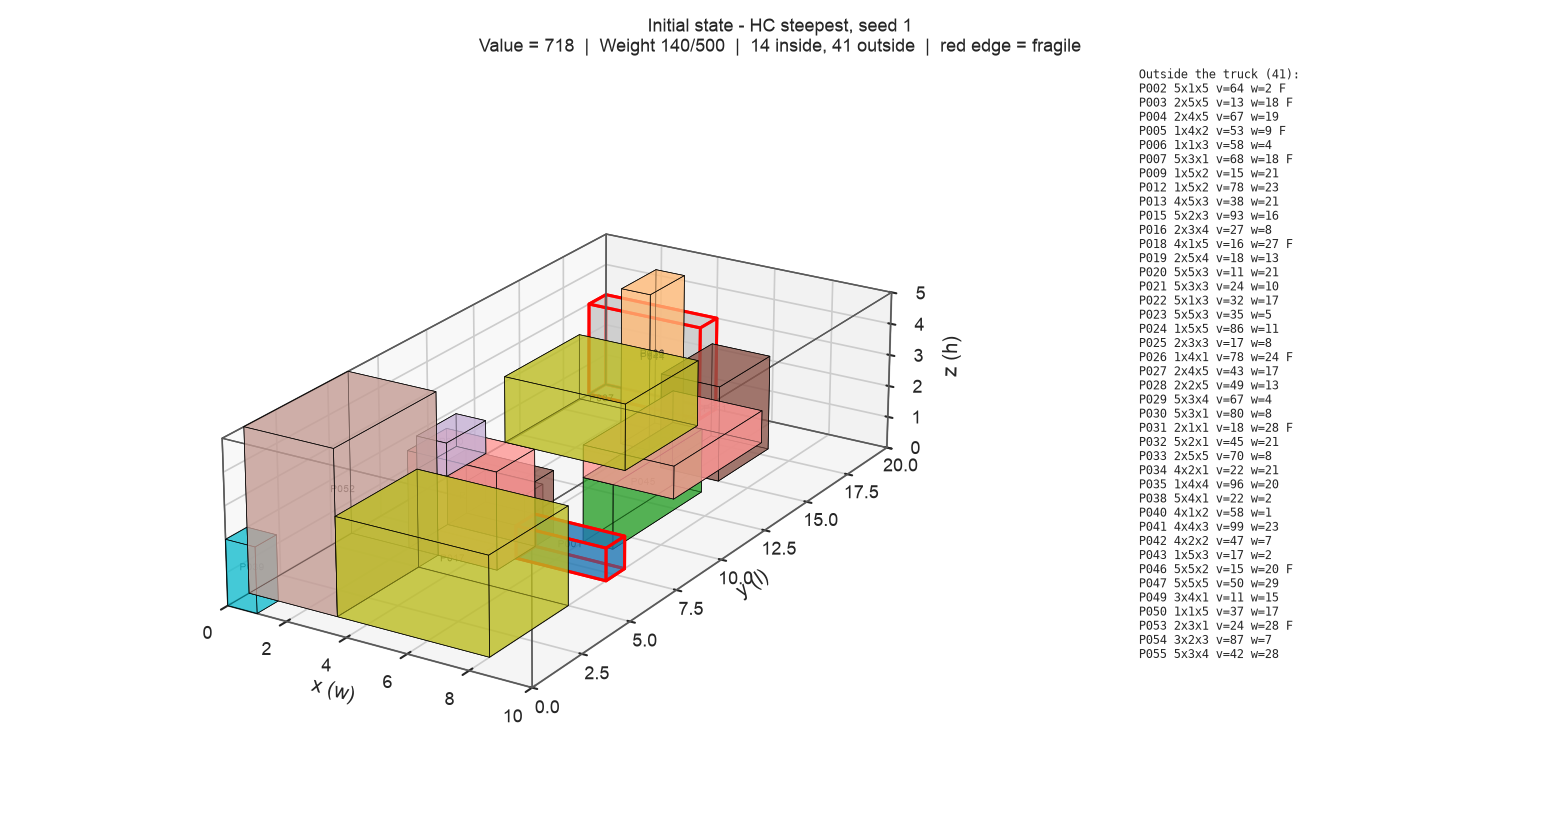
\includegraphics[width=\textwidth]{hc/medium/steepest/seed1/initial.png}
		\caption{\textit{State} awal}
	\end{subfigure}
	\begin{subfigure}{0.49\textwidth}
		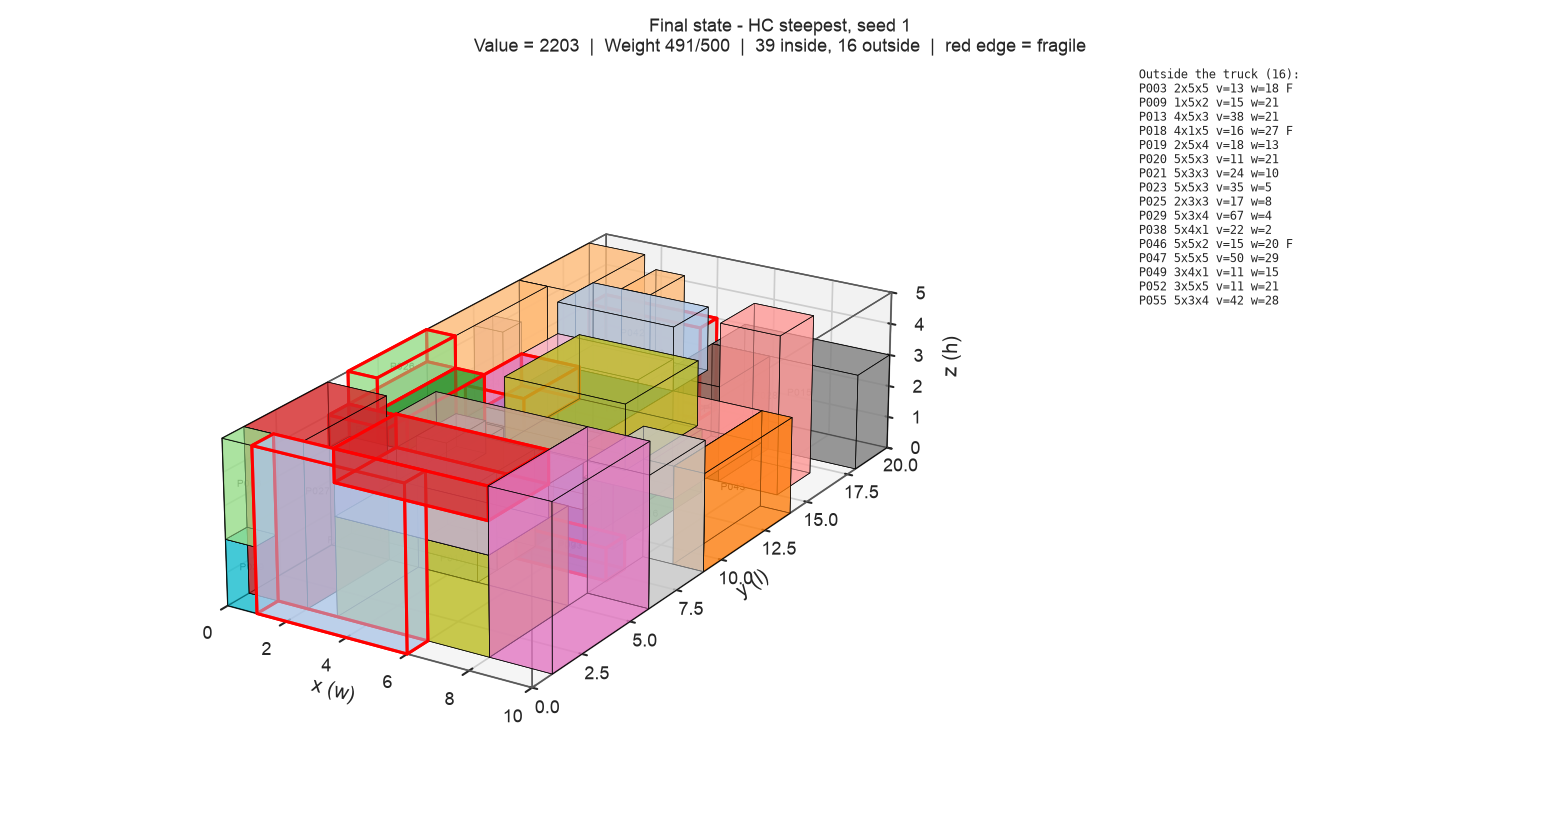
\includegraphics[width=\textwidth]{hc/medium/steepest/seed1/final.png}
		\caption{\textit{State} akhir}
	\end{subfigure}
	\caption{Visualisasi \textit{state} awal dan akhir (HC \textit{steepest-ascent}, instans \textit{medium}, \textit{seed} 1)}
	\label{fig:render}
\end{figure}

Program dijalankan melalui \texttt{src/main.py} untuk satu kali \textit{run}, misalnya:
\begin{lstlisting}[language=bash]
python -m src.main hc --instance data/instances/medium.json --variant steepest --seed 1
python -m src.main sa --instance data/instances/medium.json --iters 20000 --p0 0.01
python -m src.main ga --instance data/instances/medium.json --pop 50 --gens 100
\end{lstlisting}
Eksperimen lengkap dijalankan dengan modul \texttt{src.experiments.hc\_experiment}, \texttt{sa\_experiment}, dan \texttt{ga\_experiment}.
